%-------------------------------------------------------------------------------
% seq66 windows
%-------------------------------------------------------------------------------
%
% \file        seq66 windows.tex
% \library     Documents
% \author      Chris Ahlstrom
% \date        2021-02-13
% \update      2023-10-17
% \version     $Revision$
% \license     $XPC_GPL_LICENSE$
%
%     Provides a discussion of starting up Seq66 in Windows.
%
%-------------------------------------------------------------------------------

\section{Seq66 In Windows}
\label{sec:windows}

   This section discusses installing and using the basics of \textsl{Seq66}
   in \textsl{Microsoft Windows}.  Additional trouble-shooting information can
   be found in the installed file data directory.

   \begin{verbatim}
      C:/Program Files/Seq66/data/readme.windows
   \end{verbatim}

   Another useful reference is \cite{windowsmidi}.

\subsection{Windows / Seq66 Installation}
\label{subsec:windows_seq66_installation}

   For \textsl{Seq66}, the installer executable is now part of
   each "major" release (currently 0.99.6).
   There are tricks to getting the installer
   (e.g. \texttt{seq66\_setup\_0.99.6-x64.exe}) properly. 
   One can't just right-click and save the link.
   Instead, click on the link.  Then look for a "Download" button, and
   click that.

   Installation itself is straightforward.  Run the installer (e.g.
   \texttt{seq66\_setup\_0.99.6-x64.exe}).  Accept the license terms
   (\textsl{GNU GPL 2 or 3}),
   make sure all components are selected, accept the default
   install directory, and click through until the installation is done.

   (Note that there might also be a
   \texttt{qpseq66-release-package-0.99.6.7z} portable installer
   than can be downloaded.
   If not, request one!
   Just extract that file where desired.
   Note that the \textsl{Windows} version is a 64-bit
   application. We do not currently build a 32-bit version, due to
   our lack of a 32-bit Windows platform.)

   \textsl{Seq66} is installed at
   \texttt{C:/Program Files/Seq66/qpseq66.exe}.
   One might want to create a desktop shortcut or a shortcut button on
   the \textsl{Quick Launch} bar; one can also go to the
   "Start" menu and search for "qpseq66.exe" or "Seq66".)

   Before we discuss usage, we have to talk a bit about a Windows issue.

\subsection{Windows / MIDI Mapper}
\label{subsec:windows_midi_mapper}

   \index{windows!midi mapper}
   Windows has a \textbf{MIDI Mapper}.
   This is a subsystem that redirects MIDI to a specific device.
   Supposedly it was removed in Windows 8 and beyond, but it still
   exists in Windows 10.
   However, the alleged Control Panel applet
   for the MIDI Mapper no longer exists.

   In the Windows XP era, MIDI was exposed in the OS, 
   and it had a setup applet in the
   \textsl{Sound and Multimedia}
   \textsl{Control Panel}.
   Users could select a default MIDI Out device from a list of all
   installed MIDI devices.
   All programs outputting a MIDI data stream
   (and no selected a specific MIDI Out device)
   played their stream to that device.

   The MIDI Mapper is not real device but a "pipe";
   it receives MIDI on input and sends it to an user-configured
   MIDI Out device.
   It was bundled with Windows, installed as MIDI Out device 0, preconfigured
   to use the first available device, the built-in
   \textsl{Microsoft GS Wavetable Synth}.
   It is a low quality software wave synth, installed as MIDI Out device 1.
   So on Windows, programmers had 2 well-known devices.

   This works for MIDI software without a configurable output device; they
   use MIDI Out 0, and the wavetable synth generates the sound.
   This chain worked well: default users had working MIDI synthesis
   out of the box.
   Then Microsoft removed it in Windows 7.
   But it resurfaced in Windows 10, but without the
   MIDI Control Panel applet.

   It gets more interesting.
   Assume we have a LaunchPad Mini and a Korg nanoKEY2 plugged in.
   Internally, Windows see the following devices (based on a trek
   in the debugger):

   \begin{itemize}
      \item \textbf{0}. MIDI Mapper.
      \item \textbf{3}. GS Wavetable Synth.
      \item \textbf{4}. NanoKEY2.
      \item \textbf{5}. LaunchPad Mini.
   \end{itemize}

   Our "portmidi" implementation opens them in the same order, but
   numbers them sequentially:

   \begin{itemize}
      \item \textbf{0}. MIDI Mapper.
      \item \textbf{1}. GS Wavetable Synth.
      \item \textbf{2}. NanoKEY2.
      \item \textbf{3}. LaunchPad Mini.
   \end{itemize}

   The MIDI Mapper, if present, grabs the wavetable synth, which prevents
   \textsl{Seq66} from opening it.
   So the \textsl{Seq66}
   code detects that the MIDI Mapper (port 0) exists, and when opening
   the wavetable synth (port 1) fails, it marks that port as
   "unavailable" and "locked", in order to ghost it in the user-interface
   and ignore it for error reporting (otherwise every startup would bring
   up an annoying and meaningless error message).

   As an aside, for MIDI input, Windows does no mapping, and there are
   only two input devices (given the two plugged in above).

   \begin{itemize}
      \item \textbf{0}. NanoKEY2.
      \item \textbf{1}. LaunchPad Mini.
   \end{itemize}

   There are applications that try to get around this issue, such as
   the \textsl{CoolSoft MIDIMapper} and \textsl{VirtualMIDISynth}
   \cite{midimapper} or \textsl{MIDI OX} \cite{midiox}.
   See the \texttt{readme.windows} file for more information.

\subsection{Windows / Virtual Ports}
\label{subsec:windows_virtual_ports}

   Virtual ports are software MIDI ports that can be created for
   input and output, as noted in
   \sectionref{paragraph:menu_edit_preferences_midi_clock} and
   \sectionref{paragraph:menu_edit_preferences_midi_input}.
   To provide virtual ports in \textsl{Windows},
   special software needs to be installed.
   One useful applications is \textsl{LoopMIDI} (see \cite{loopmidi}).

   \begin{quote}
      Virtual loopback MIDI cable for Windows 7 up to Windows 10, 32 and 64
      bit.  This software can be used to create virtual loopback MIDI-ports to
      interconnect applications on Windows that want to open
      hardware-MIDI-ports for communication.
   \end{quote}

   With this software, one can create a number of extra MIDI ports.
   The main difference from \textsl{Linux} here is that the
   \texttt{--manual-port} option is \textsl{not} used.
   The virtual ports are treated as real ports in \textsl{Windows}.

\subsection{Windows / Seq66 Startup}
\label{subsec:windows_seq66_startup}

   Now run \texttt{C:/Program Files/Seq66/qpseq66.exe}.
   It might generate an error, though we believe we have suppressed
   this error:

\begin{figure}[H]
   \centering 
   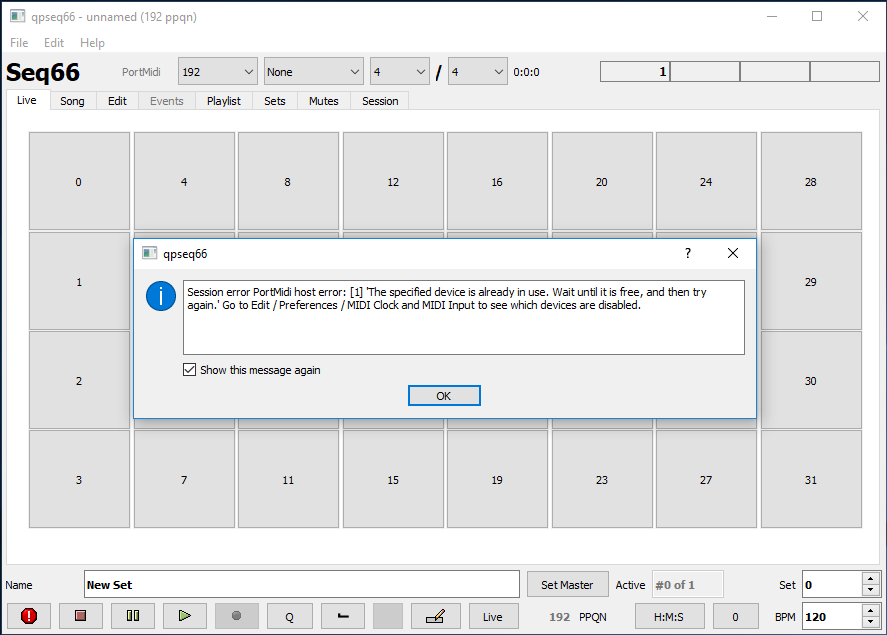
\includegraphics[scale=0.65]{windows/windows-first-startup.png}
   \caption{Seq66 First Startup in Windows}
   \label{fig:windows_first_startup}
\end{figure}

   This error occurs on \textsl{Windows 10} because the 0th port, the
   \textsl{Microsoft MIDI Mapper}, grabs access to the 1st port, the
   \textsl{Microsoft GS Wavetable Synth}.
   Thus, the wavetable synth is "unavailable" and "locked".
   This message will appear at startup for "unavailable" ports,
   but not for a "locked" port; one can also just click
   \textbf{OK}, but startup messages can also be suppressed using an option in
   \textbf{Edit / Preferences / Display}.

   Run the \textsl{qpseq66.exe} shortcut and load a tune from the
   directory \texttt{C:/Program Files/Seq66/data/midi}.

   Navigate in the file explorer to
   \texttt{C:/Users/your\_user\_name/AppData/Local/seq66} and open
   \texttt{qpseq66.rc}, the main configuration file for \textsl{Seq66}.
   It will look like this:

\begin{figure}[H]
   \centering 
   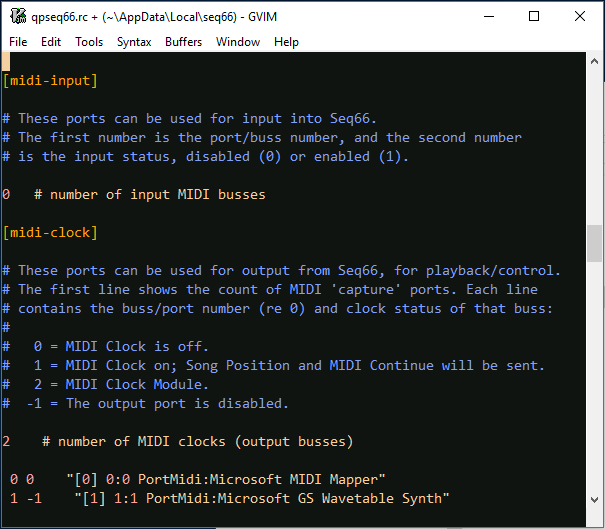
\includegraphics[scale=0.75]{windows/rc-file-post-first-startup.png}
   \caption{'rc' File After Exiting First Startup}
   \label{fig:windows_rc_file_post_first_startup}
\end{figure}

   The \texttt{[midi-input]} section indicates there are no input ports
   in Windows when no MIDI device is connected to the computer.
   The \texttt{[midi-clock]} section indicates there are two output
   ports, and that port 1 is disabled.   So one should be able to
   play a tune to the MIDI Mapper and hear it, if output is directed
   to port 0.

   Go to \textbf{Edit / Preferences / MIDI Clock}.
   It will look like this:

\begin{figure}[H]
   \centering 
   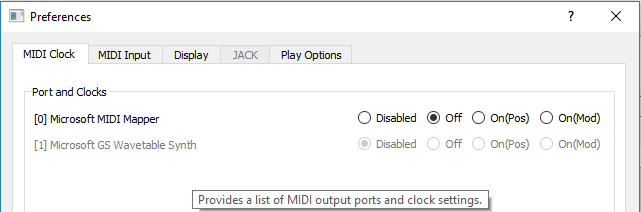
\includegraphics[scale=0.85]{windows/edit-preferences.png}
   \caption{MIDI Output Settings at Second Startup}
   \label{fig:windows_output_settings_second_startup}
\end{figure}

   Next select \textbf{File / Open} and select this sample tune:

   \begin{verbatim}
      C:/Program Files/Seq66/data/midi/b4uacuse-gm-patchless.midi
   \end{verbatim}

   (In the following figure, the " (x86)" is due to an early incorrect
   installation; \textsl{Seq66} on Windows is a 64-bit application only
   at this time.)

\begin{figure}[H]
   \centering 
   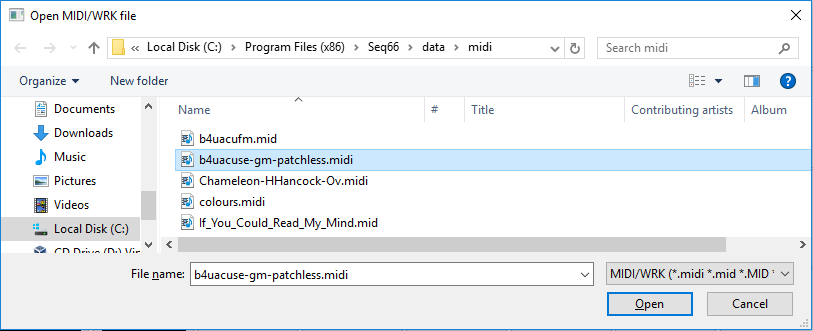
\includegraphics[scale=0.65]{windows/open-installed-midi-file.png}
   \caption{MIDI File Selection}
   \label{fig:windows_open_installed_midi_file}
\end{figure}

   After clicking \textbf{Open}, the following set of patterns is shown.
   Note the two highlighted areas, "Output Selector" and "Song/Live Button".

\begin{figure}[H]
   \centering 
   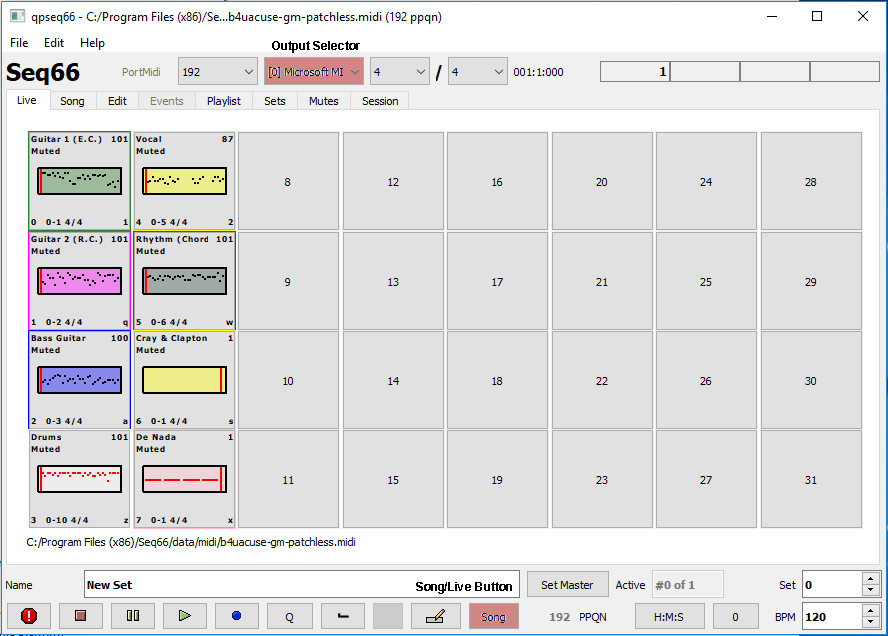
\includegraphics[scale=0.65]{windows/open-midi-file.png}
   \caption{Opened MIDI File}
   \label{fig:windows_open_midi_file}
\end{figure}

   At the top, select port 0 (the MIDI Mapper) from the "Output Selector".
   This \textsl{modifies} the MIDI file so that all MIDI
   output will go to port 0.

   At the bottom, click the "Song/Live Button" until it reads "Song".
   This will access track layouts that turn on all of the patterns.
   These layouts can be seen by selecting the \textbf{Song} tab.

   Now click the play button (green triangle).
   The song should play properly.
   (On our test Windows 10 setup in a virtual machine, playback is ragged,
   but fine on a normal Windows installation on hardware.)

   Overall, the \textsl{Windows} version and the \textsl{Linux} version
   work essentially the same. The \textsl{Linux} version can use the
   \textsl{ALSA} and \textsl{JACK} MIDI engines, while the \textsl{Windows}
   version uses a refactored \textsl{PortMidi} engine that is part of the
   \textsl{Seq66} project.

   The \textsl{PortMidi} engine should also work with \textsl{MacOSX}, but,
   since we don't have a Mac, we haven't been able to build and test
   on that platform.
   Again, for trouble-shooting, also see the installed text file:

   \begin{verbatim}
      C:/Program Files/Seq66/data/readme.windows
   \end{verbatim}

\subsection{Windows / Keyboard Issues}
\label{subsec:windows_keyboard_issues}

   The keystroke processing of \textsl{Seq66} is based on looking up
   \textsl{Qt} key scan codes and then finding the matching key modifiers (e.g.
   Shift or Ctrl) and native virtual key numbers.
   When a match is found, a \textsl{Seq66}-specific ordinal value ranging from
   0 to 255 is found, and that is used to look up the command or function
   associated with that keystroke.

   The native virtual key numbers are how the operating system
   encodes the various hardware keys on the keyboard.
   These numbers vary between
   \textsl{Linux},
   \textsl{Windows}, and
   \textsl{Mac}.
   All these numbers are in a table, and there is (currently)
   a table for \textsl{Linux} and a table for \textsl{Windows}.

   The table for \textsl{Windows} was recently completed, but
   it is likely that there are some native virtual key numbers
   that were not assigned correctly.
   Report any issues.

   There is also a table that corrects for
   \index{keys!AZERTY}
   the French AZERTY layout.
   It is a good bet that this table also has errors.
   Report any issues.

%-------------------------------------------------------------------------------
% vim: ts=3 sw=3 et ft=tex
%-------------------------------------------------------------------------------
